\chapter{Materials and Methods}\label{chap:methods}
The challenges in genomic analysis of viral material using NGS raw read data are the major motivation for this thesis. Ready-to-use pipelines that can be executed without deeper biological or bioinformatical knowledge specifically designed for the viral genomes of avian influenza, pox and foot-and-mouth disease are presented below. They run on the Galaxy platform and show that for development of the pipelines, large parts of existing viral genomic analysis pipelines as such for SARS-CoV-2 can be reused and adapted.

\section{Galaxy Platform}\label{sec:galaxy}
Galaxy is a web-based scientific platform that has become a major player in many fields of life sciences and bioinformatics. Founded in 2007, it has provided an emerging amount of resources and tools to empower scientists and researchers to work with biomedical datasets. The platform is free to use and collaborative, as all related codebases are open-sourced on GiHub. Resources on Galaxy cover genomics, metagenomics, transcriptomics, proteomics, drug discovery and non-biology fields like natural language processing and social sciences.

Galaxy's primary objective is to make analyses more accessible, reproducible, and easier to communicate among researchers. The platform's distinctive and success is attributed to four core elements: a very active community, a public server for analyses, an open-source software ecosystem, and the Galaxy ToolShed. The community adheres to the FAIR practises (Findable, Accessible, Interoperable and Reusable)~\cite{10.1093/nar/gkac247}.

The Galaxy community is thriving, with over 124,000 users who also contribute to subcommunities. The public server for analyses provides access to public datasets and workflows. The open-source software ecosystem ensures automated setup and deployment of all tools and services, making it simple for beginners and professionals to use. The Galaxy ToolShed is a server dedicated to hosting, sharing, and installing tools used on the platform. A Galaxy tool is the abstraction layer that makes external software usable from within Galaxy with a frontend, i.e. lets users use the program with all its parameters and inputs from within Galaxy. Each program that is available as a Galaxy tool is XML-wrapped to make dependency requirements, parameter and data inputs and other settings possible via the Galaxy web-interface. \\ 
Galaxy workflows are a key feature that allow the user to stack tools in a chain and to configure them so that the workflow user only has to upload or enter data for the input fields. The automated subsequent order and execution of tools in a workflow is used for modular, longer analyses that are executed repeatedly. Each user gets 250 GB of disk space to run computations. \\
Workflows that are available on and accepted by the \ac{IWC} on GitHub are conform with the community's best practise standards and tested on the latest Galaxy release. Dockstore for availability in the US and WorkflowHub for EU users  publish the \ac{IWC} workflows and guarantee the availability in Docker-based environments~\cite{o2017dockstore} and on the workflow collaboratory WorkflowHub~\cite{goble2021implementing}.

Important contributions of Galaxy, as stated by the Galaxy Community (2022), include Vertebrate Genome Project assembly workflows and research collaborations about \ac{SARS-CoV-2}. Another toolkit leveraged in Galaxy is Galaxy-ML, a set of tools that form a suite for analyses based on machine learning. With growing publicity, more topics are covered by and moved to Galaxy. It has contributed to over 5,700 scientific publications and has many tutorials available for researchers to use. \\
The Galaxy platform is continuously enhanced, and it still attracts around 2,000 new users every month, indicating its quality and significance. The team and infrastructure of Galaxy initially come from the Nekrutenko lab in the Center for Comparative Genomics and Bioinformatics at Penn State, the Taylor lab at Johns Hopkins University, and the Goecks Lab at Oregon Health \& Science University. There are 138 public servers available worldwide as of 2023, while the most prominent general-purpose server instances are hosted by teams at University of Freiburg, Germany for \href{https://usegalaxy.eu/}{UseGalaxy.eu}, Texas Advanced Computing Center for \href{https://usegalaxy.org/}{UseGalaxy.org} and Genomics Virtual Laboratory, formerly at the University of Queensland for \href{https://usegalaxy.org.au/}{UseGalaxy.org.au}. These public servers are synchronised in a set of reference tools~\cite{10.1093/nar/gkac247}. \\
The platform serves as a public infrastructure that can be used in many different contexts and by professionals from all fields and backgrounds. It therefore is very suitable for offering publicly available and transparent resources for surveillance of diseases.

\section{SARS-CoV-2 Workflow and Requirements}
The \ac{COVID-19} pandemic motivated many researchers to study and develop analysis workflows of \ac{SARS-CoV-2} sequencing data. In the \ac{IWC} repository, there are seven workflows available and ready to use on Galaxy for the different kind of NGS data (ONT/Illumina) and with varying objectives (variant calling/variation reporting/consensus construction). Specifically for Illumina ARTIC reads, a workflow for genomic analysis based on the \texttt{iVar} suite has been released~\cite{iwc2021covidivar}. It is conceptually similar to other existing pipelines outside of Galaxy, written in Nextflow, Snakemake and \ac{WDL}. The workflow for ampliconic Illumina paired-end reads consists of the following steps: (1) read adapters are trimmed with \texttt{fastp} and (2) mapped to a reference genome with \texttt{BWA-MEM}. The alignment is (3) quality filtered using \texttt{Samtools view}, keeping the reads with a minimum length of 20 and only if they are mapped and properly paired. After generating quality and coverage reports, (4) \texttt{iVar trim} is run with the primer scheme to cut out the primers from the filtered alignment. The cleaned alignment file is processed (5) with \texttt{iVar consensus} to call the consensus sequence and (6) with \texttt{iVar variants} to call variants. The resulting outputs are used for variant annotation, phylogenetic assignment of the outbreak lineages and clade assignment. The structure of the workflow is depicted in~\figref{fig:3-sars-wf}. 

\begin{figure}[h!]
	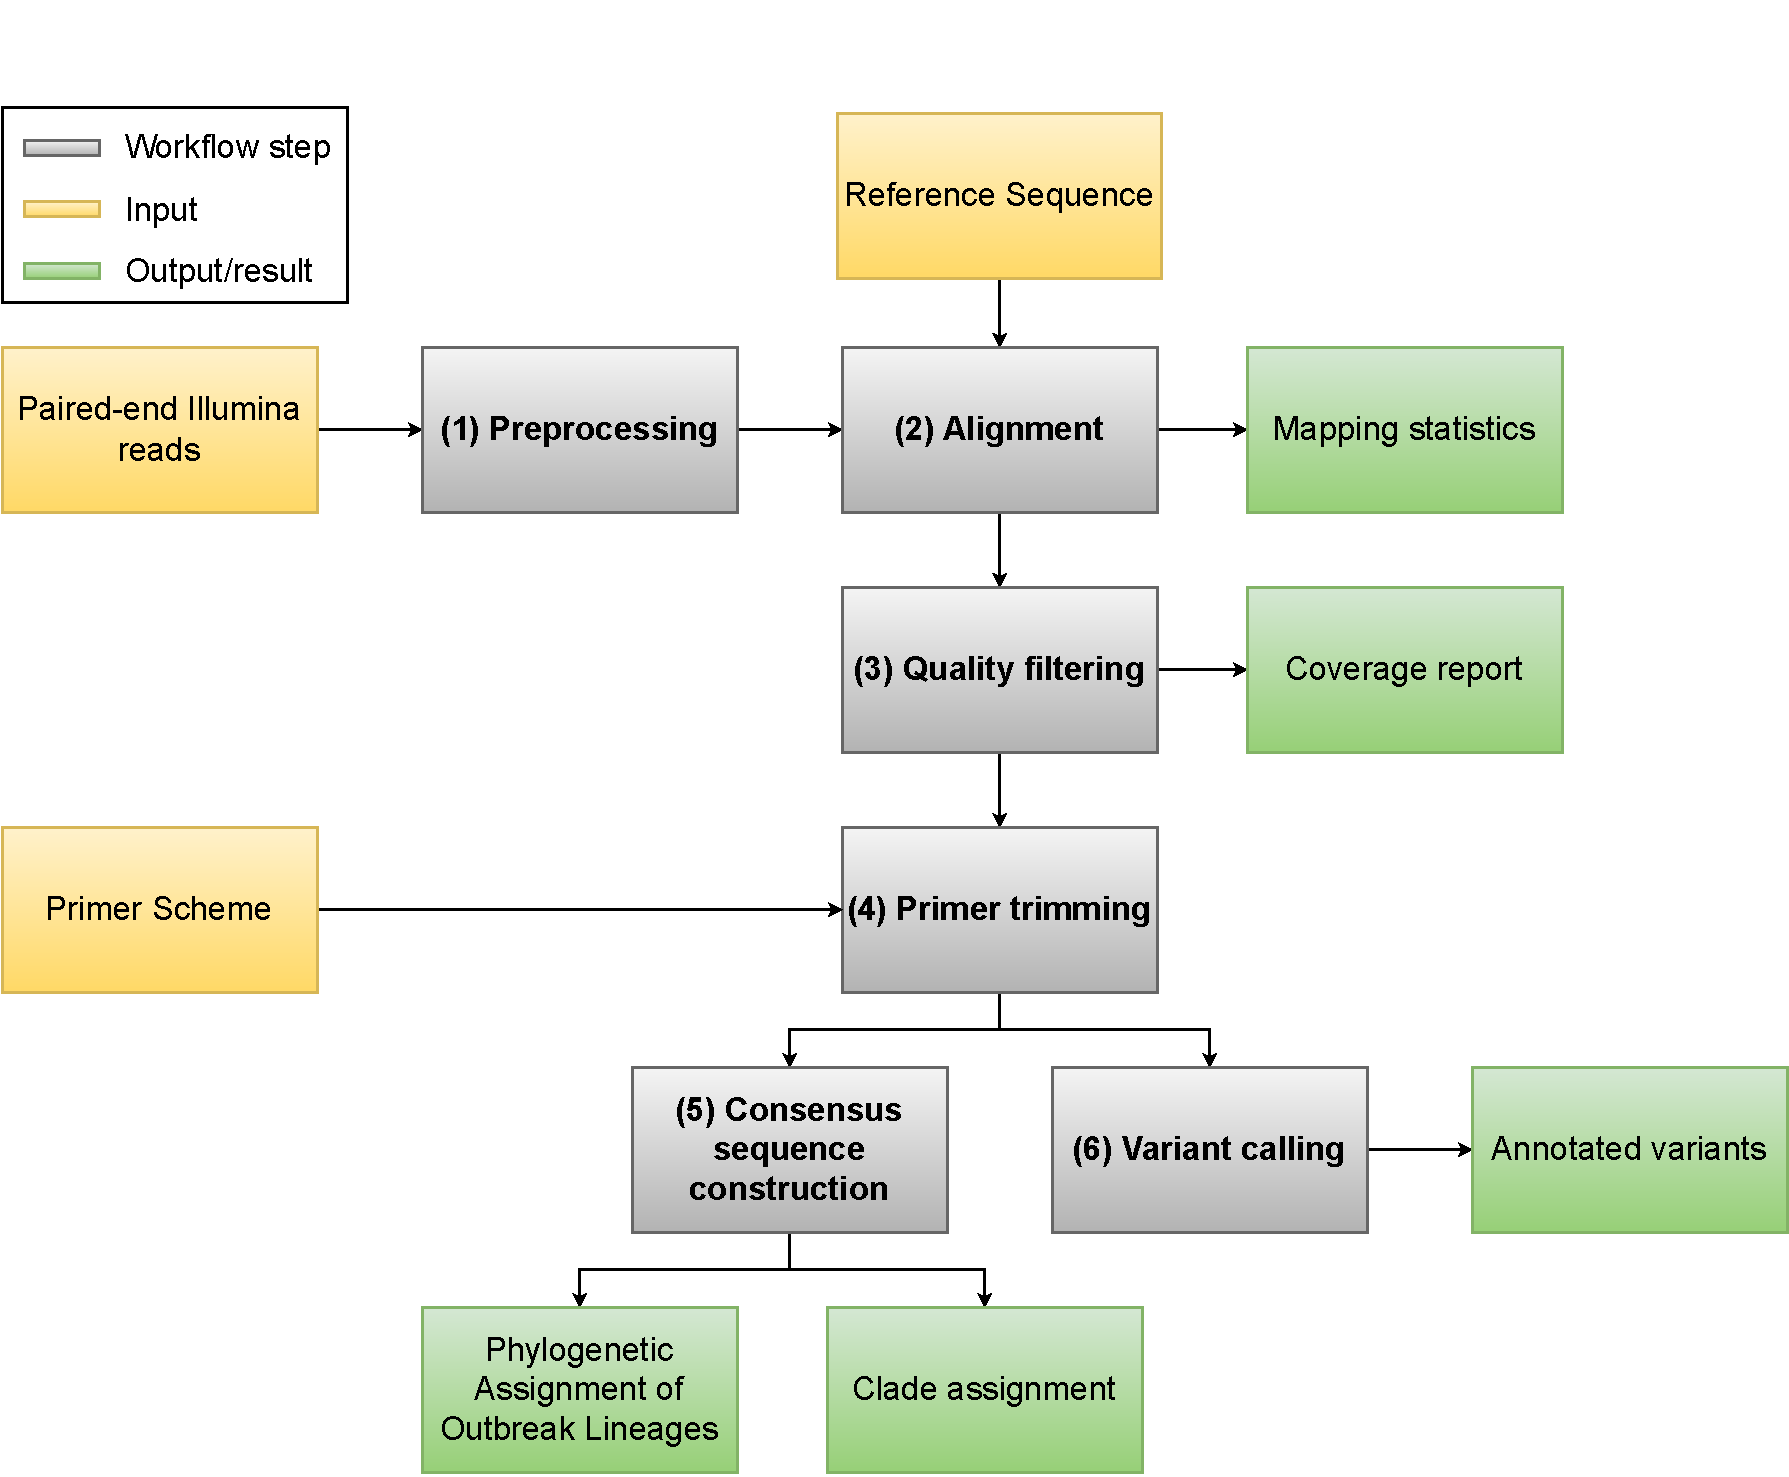
\includegraphics[width=0.95\textwidth]{media/3-sars-cov-2.pdf}
	\caption{Simplified SARS-CoV-2 analysis workflow for ampliconic Illumina-sequenced data.}
	\label{fig:3-sars-wf}
\end{figure}

This workflow is designed for the specifics of the SARS-CoV-2 genome, however most viral genomes can be analysed in similar ways. Accounting for the genomic structure and composition of each virus, analysis workflows for poxviruses, avian influenza virus and foot-and-mouth disease virus are developed, reusing modified components of the described \ac{SARS-CoV-2} worfklow. The requirements for the viruses and the workflows are described below, before the developed workflows are examined. %% more

\subsubsection{Requirements for Poxvirus Analysis Workflow}
As explained in~\secref{sec:2-pox}, the genome of most poxviruses is bound by identical sequences located at the termini of the genome. It is shown that the size of such differs for some poxviruses, such as rabbitpox and vaccinia virus, while monkeypox, cowpox and capripoxviruses have shorter \acp{ITR}~\cite{wittek1978inverted}. For a whole-genome reconstruction from \ac{HTS}-generated reads, alignment algorithms look for the unambiguous location of a read. Since this is impossible for repeated identical sequences neither for reference-based mapping approaches nor \textit{de novo} assembly, a new approach has to be used that splits the sequencing reads into two parts, separating the identical sequences and running alignment algorithms for each of the splits. To build the full-length genome, the alignments need to be ``glued'' together. This approach requires the reads to be sequenced in two pools with two libraries. A similar protocol has been described by Mathijs et al. and the ARTIC network for SARS-CoV-2 data~\cite{mathijs2022robust, tyson2020improvements}. \\
As a consequence, a requirement for a reference-based surveillance of the genomics of poxviruses is the availability of the primer scheme that was used for amplicon-based sequencing with an Illumina sequencer. The \ac{BED} file containing the primers, their positions and the pool identifier is essential for the correct linking of the alignments when splitting the pipeline into two parts and merging it back together. \\
Apart from the split approach with a masked reference sequence for alignment, the poxvirus reads can be processed in the same way as \ac{SARS-CoV-2} reads. In the \ac{SARS-CoV-2} workflow, clade and lineage assignment, with \texttt{Nextclade} and \texttt{Pangolin} respectively, work with \ac{SARS-CoV-2} specific databases. Although the tools are designed to work with the \ac{SARS-CoV-2} genome, the \texttt{Nextclade} tool is adapted and expanded to work with other viruses (mpox, Influenza A H1N1 and H3N2 HA gene, Influenza B Victoria and Yamagata HA)~\cite{aksamentov2021nextclade}.

\subsubsection{Requirements for AIV Analysis Workflow}
The main objectives of surveillance of \ac{AIV} on the genetic level are to get phylogenetic insights and to check for new variants that could occur in the \ac{HA} and \ac{NA} proteins as a consequence of reassortment. \\
A pipeline for an avian influenza virus sample that should build a consensus sequence in order to check for mutations needs a reference sequence that it can align the sequence to. A main caveat of many existing pipelines is the user's choice of reference sequence, since it is an arbitrary choice, and it has a direct impact on the alignment. The goal is to pick a reference that is representative of the sample being analysed. In the \ac{SARS-CoV-2} pipeline, a reference genome is recommended from a recent strain. For avian influenza virus, multiple reference sequences exist depending on the strain and subtype. Hence, a dynamic approach that is sensitive enough for the segmented structure of the \ac{AIV} genome is needed to pick a representative reference. The diversity of \ac{HA} and \ac{NA} segments' sequences is significant enough to make it challenging to map sequenced reads to a single, full-length influenza A reference sequence. Although this approach may be effective for the other six segments, the mapping software would frequently be unable to locate sufficient plausible matches for sequenced reads of \ac{HA} and \ac{NA} origin to continue with the analysis. By using a split approach that finds the best reference sequence from a database, the expensive assembly step is avoided and mapping to a suitable reference can be conducted. \\
Compared to analyses with genomes such as \ac{SARS-CoV-2} and due to the segmented structure of the \ac{AIV} genome, duplicates among the mapped reads of the \ac{AIV} sample should not be dismissed but kept for maintaining a reasonable high coverage for the further analyses. Downstream analyses for phylogenetic placing are useful for the \ac{HA} and \ac{NA} genes, as well as visual summaries of \acp{SNP} to identify genetic variation in different regions.

\subsubsection{Requirements for FMDV Analysis Workflow}
The non-segmented structure of the relatively short \ac{FMDV} viral genome allows for a straight-forward analysis and reconstruction of the full-length genome by consensus sequence construction. Similar to the workflow for \ac{AIV}, a dynamic reference search from a database helps to find the best reference genome for alignment. Otherwise, reference-based mapping and consensus sequence construction as well as quality and coverage reports are processed in the same way as in the \ac{SARS-CoV-2} workflow. Although the genomes of \ac{FMDV} and \ac{SARS-CoV-2} are of different lengths, both can be analysed in a very similar way. For the developed \ac{FMDV} workflow, genomic sequencing data are required.

\section{Workflow Development}
Galaxy workflows developed for poxviruses, \ac{AIV} and \ac{FMDV} that account for the genomic structure of each virus and the NGS approaches are described below.

\subsection{Poxvirus Illumina Amplicon Workflow}\label{sec:pox-wf}
The proposed Galaxy workflow for poxvirus samples that were Illumina-sequenced with a tiling amplicon approach is available on WorkflowHub, Dockstore and on \ac{IWC} to use on Galaxy EU (links in Supplementary~\secref{sec:apx-pox-links}). \\
This workflow is the first public pipeline for ampliconic Illumina-sequenced data that provides a ready-to-use infrastructure for genomic analysis of poxviruses with a tiled amplicon approach. It aims at constructing the full genome from ampliconic Illumina-sequenced reads and providing alignment files, consensus sequence and intermediate results and reports that give insights into reads, mapping quality and mapping coverage. An overview of all steps, these outputs and the respective datatypes in \ac{CWL} \todo{?} is provided in the Supplementary~\secref{sec:apx-pox-wf}. The pipeline is clearly and summarised shown in~\figref{fig:3-pox-wf}. \\ 
To account for the repeated \acp{ITR} at the ends of the poxvirus genome, the workflow is based on a tiled amplicon approach. During the first steps, the reads of the two pools from each genome half are processed individually as half genomes. Input data for the workflow are two distinct collections of reads from \textit{pool1} and \textit{pool2}, sourced from the sequencing with two libraries; the used primer scheme in \ac{BED} file format that contains an indicator for \textit{pool1} or \textit{pool2} in the \textit{SCORE} column, and a reference sequence that is used for mapping. 

\begin{figure}[ht!]
	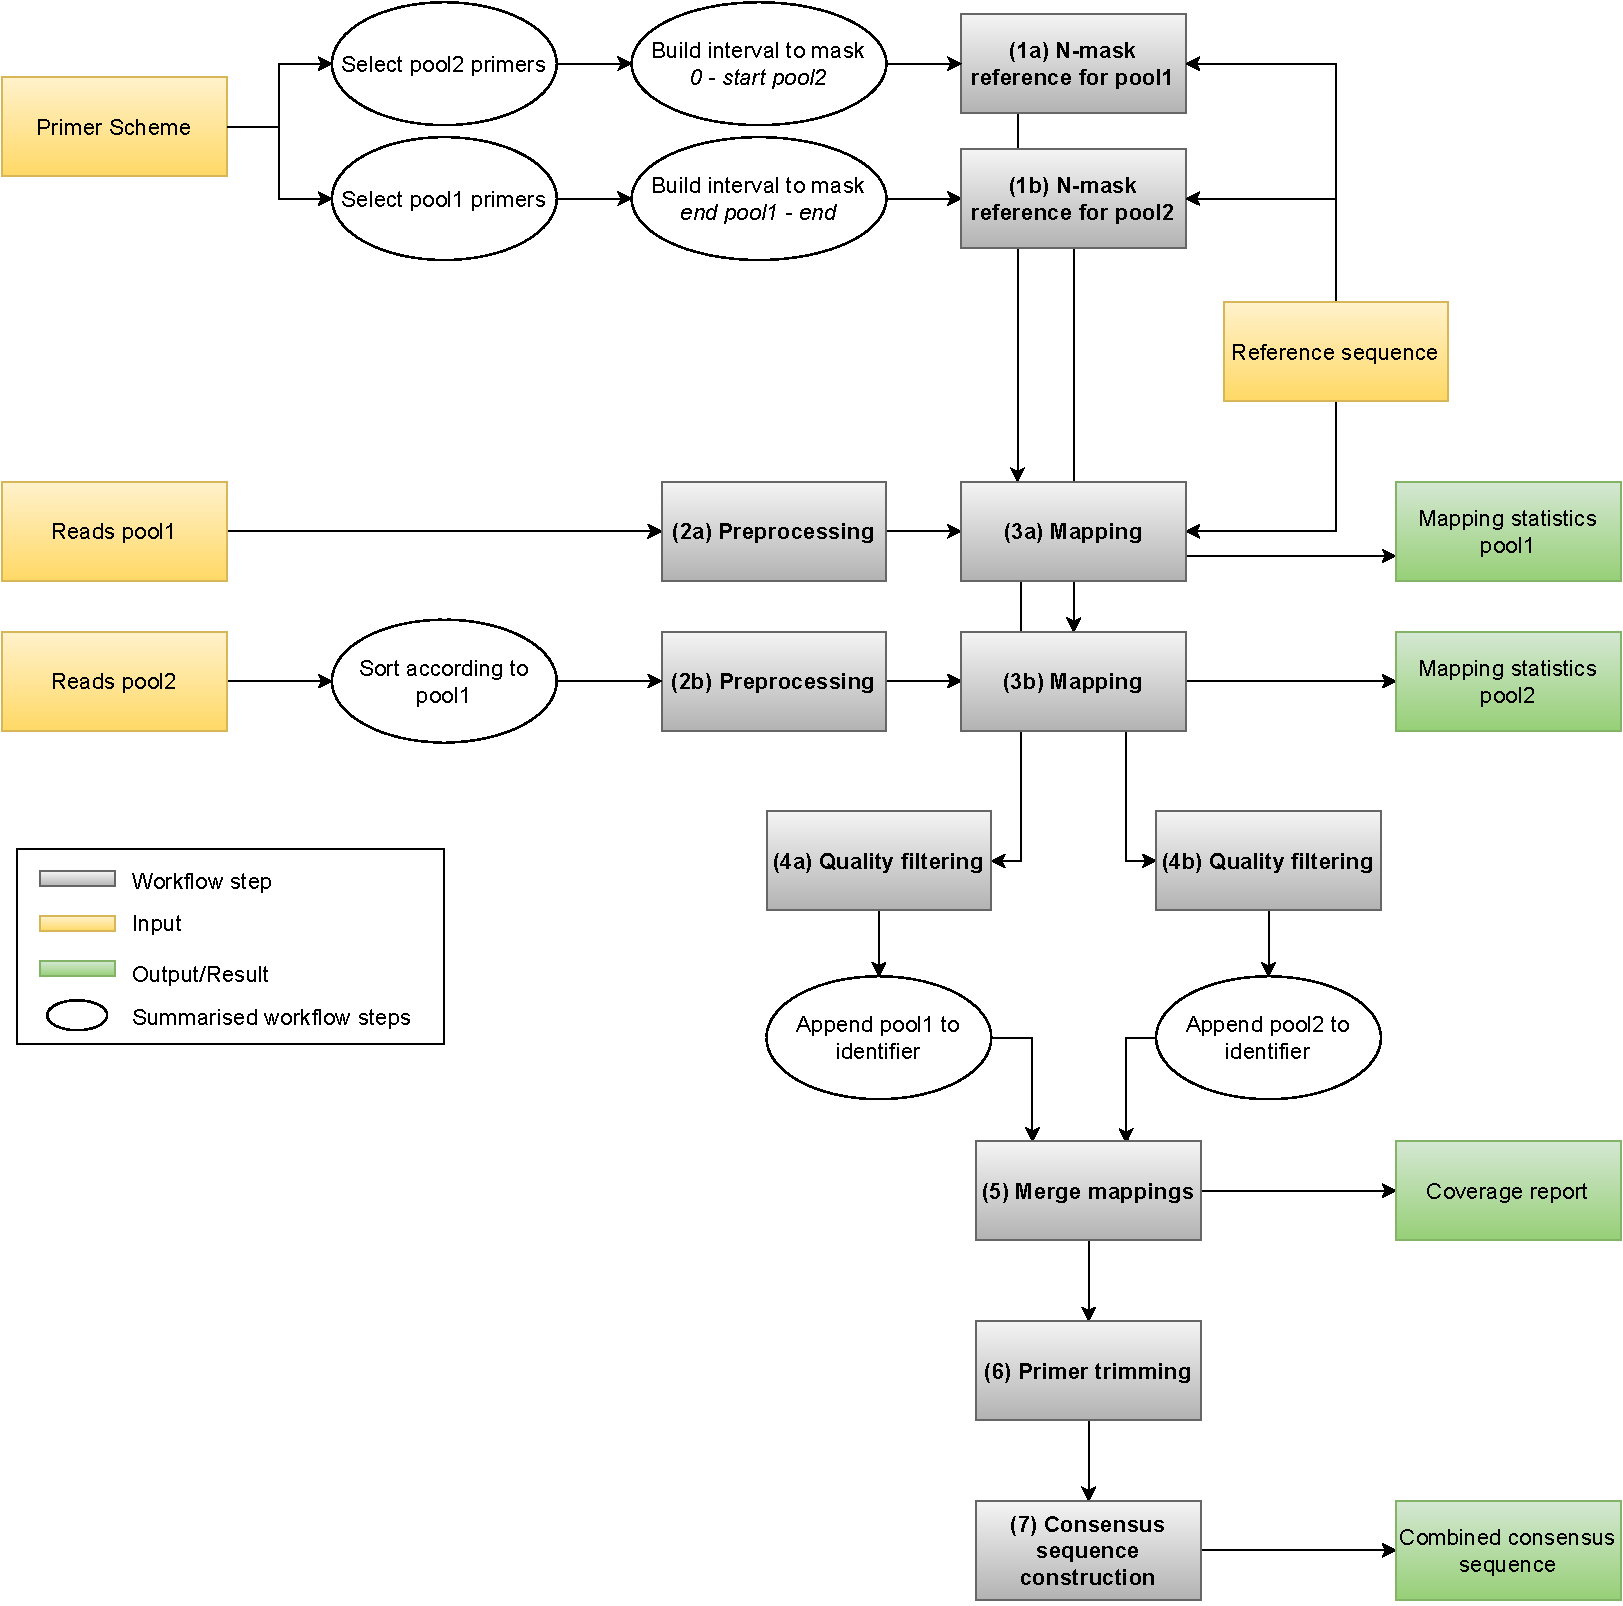
\includegraphics[width=0.92\textwidth]{media/3-pox.pdf}
	\caption{Simplified poxvirus genomic analysis workflow for ampliconic Illumina-sequenced data.}
	\label{fig:3-pox-wf}
\end{figure}

As a first step, (1) the provided reference sequence is prepared for the mapping of the two read pools. Hence, the primer scheme is needed to determine the exact start and end position of the pools so that the remaining bases are N-masked. For mapping \textit{pool1} against the full-length reference, the second half of the reference sequence is N-masked and therefore the interval for the remaining bases is constructed as a text parameter. The masking starts at the minimal start position of the first primer of \textit{pool2}. If the pools and primers are of similar size, this position is in the middle part of the reference sequence. It is important that this position that separates the pools is between the \acp{ITR} so the individual mappings of each pool only contain one \ac{ITR}. Accordingly for the mapping of \textit{pool2}, the interval of the remaining bases is constructed by taking the maximal end position of the \textit{pool1} primers and the full length of the reference sequence so that the masking of the first half can be conducted. The construction of the text parameter in the correct input format is done by multiple Galaxy-specific text-processing tools% and can be looked up in the Supplementary~\tabref{tab:aiv-tools-steps}.
Using this approach, it is ensured that the \acp{ITR} are unambiguously mapped and coverage statistics are expressive, which would not be the case if mapping would be performed on the full-length reference and reads from the \ac{ITR} regions could be mapped to either one \ac{ITR}. \\
The workflow is designed to process multiple samples in one run, thus for better comparison the samples of the second pool are sorted by the order of how they are listed in \textit{pool1}. Before mapping, (2) the reads of both pools are preprocessed with \texttt{fastp} to automatically trim Illumina-specific PolyG tails of the reads. The following (3) mapping step with \texttt{BWA-MEM} takes the corresponding masked reference sequence for each genome-half. A statistics report for each alignment is generated using \texttt{Samtools stats} and allows the user to inspect the mapping quality and coverage. The alignments are (4) filtered for quality with \texttt{Samtools view} to keep reads with a minimum length of 20 and only properly paired and mapped reads. Additionally, the pool identifiers (\textit{pool1/pool2}) are prepended to the sample names so that using external software to check variants, the pool and sample identification is maintained and unambiguous. In the next step (5), the two alignments are merged while retaining the identifiers for each sample and pool. For the full-length mapping, a coverage report is generated with \texttt{QualiMap BamQC} so that the \acp{ITR} and the part where the mappings are merged can be inspected. The mean coverage depth is an important standard parameter when performing NGS. It indicates how often each base occurs on average in the individual reads. For smaller segments or amplicon-based data, checking the depth of coverage in each region is crucial as it provides information on how close the sequenced sample is to the reference sequence selected for mapping. Low coverage indicates incorrect mapping due to many genetic differences. Therefore, coverage plots are given for each sample. \\
(6) Primer-trimming with \texttt{iVar trim} removes the loose primer ends and cleans the alignment for the consensus sequence construction. The (7) consensus sequence is called with \texttt{iVar consensus} and a 10-fold minimum depth. For this step, the user can either use provided default settings (minimum quality score to count base: 20, minimum allele frequency threshold to call SNV: 0.7, minimum allele frequence to call indel: 0.8) or enter their own values before starting the workflow. These settings yield for the minimum of ten sequenced reads per base in coverage. With the final combined consensus sequence in FASTA format for each input sample, any downstream analyses can be started. \\
%The workflow with a complete list of the 47 steps, used tools with version number, settings, outputs and connections between the tools is provided in Supplementary~\tabref{tab:pox-tools-steps}. 

\subsection{AIV Illumina Workflow}\label{sec:aiv-wf}
We propose a fully automated pipeline for the analysis with a reference-based mapping approach of Illumina-sequenced paired-end reads from avian influenza samples. The workflow is integrated in the Galaxy platform and is available with all related material via links provided in Supplementary~\secref{sec:apx-aiv-links}. Furthermore, to the best of our knowledge this pipeline is the first ready-to-use workflow that uses a hybrid reference sequence for a fast mapping and provides many outputs for various downstream analyses. It is designed to take one input sample at a time and besides a summarising results report, the outputs of the analysis steps can be used for further research based on the user's interest. The workflow is outlined in~\figref{fig:3-aiv-wf}, where the nine main steps of the workflow are visualised. The full workflow of 48 steps with the tools, tool version and settings in \ac{CWL} format \todoit{?} can be found in Supplementary~\secref{sec:apx-aiv-wf}. \\
One novelty of the workflow is the consideration of the different segments of the influenza virus genome. After uploading paired-end reads and a reference sequence database, the workflow builds a hybrid reference from the given database for each of the segments of the genome. The reference sequence database consists of eight FASTA files, one per segment (PB2, PB1, PA, HA, NP, NA, M, and NS), containing multiple full-length sequences per segment. The provided database file consists of \todo{many} sequences for each segment. The reference collection is ready to import into a new history and publicly available on Galaxy EU (link in Supplementary~\secref{sec:apx-aiv-wf}). If a user decides to upload their own references, it is important to follow the sequence identifier pattern so that the extraction of sequence identifiers in the workflow works as expected: >\textit{segment\_name$\mid$influenza\_strain$\mid$subtype$\mid$accession\_number}. For example, one entry's identifier is >\textit{PB1$\mid$A/duck/Manitoba/1953$\mid$A/H10N7$\mid$KF435047.1} followed by the sequence in the next line. 

\begin{figure}[ht!]
	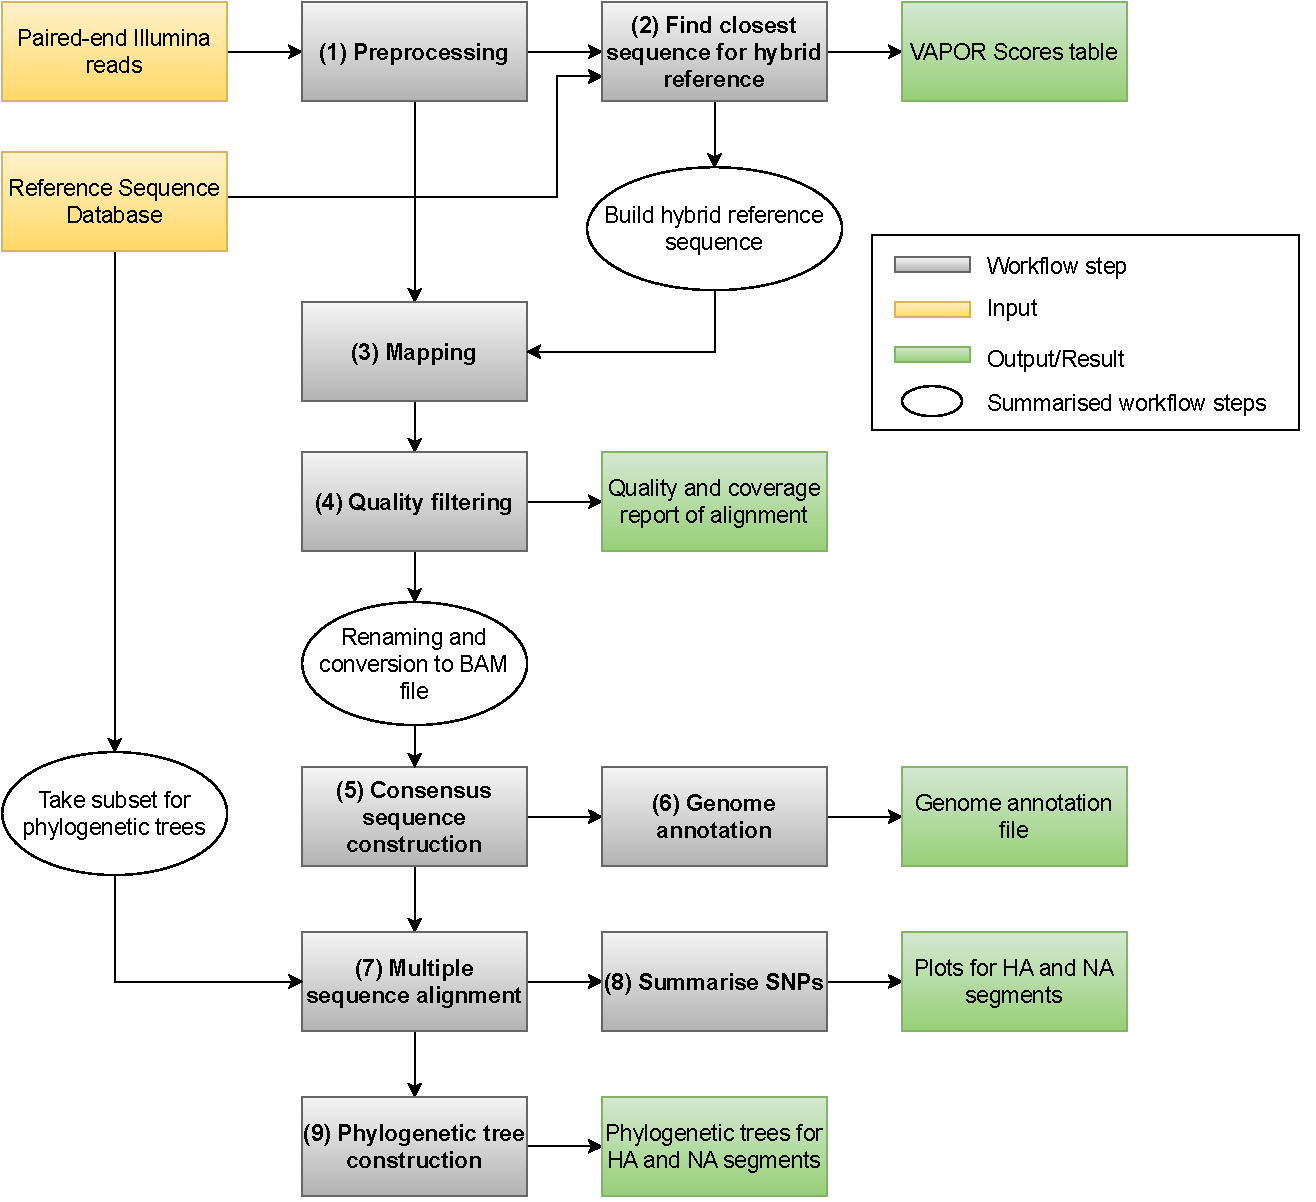
\includegraphics[width=0.9\textwidth]{media/3-aiv.pdf}
	\caption{Simplified \ac{AIV} genomic analysis workflow for Illumina-sequenced data.}
	\label{fig:3-aiv-wf}
\end{figure}

After (1) preprocessing of the reads with \texttt{fastp} to dismiss reads shorter than 30 basepairs and automatic trimming PolyG tails of the Illumina reads, the database of reference sequences is used to (2) find the closest possible reference for each of the segments. The tool \texttt{VAPOR} outputs a table with a scoring based on the weighted graph construction, and should not be confused with the identity of the sequence compared to the reference. As \texttt{VAPOR} is running once per segment but has independent inputs, this step is executed in parallel. \texttt{VAPOR} is a graph-based classifier that maps k-mers to a weighted De Bruijn graph~\cite{southgate2020influenza}. Benchmarking shows that it runs significantly faster than \ac{BLAST} and default configurations lead to reasonable matches similar to Mash, as long as the given sample is not very different from or novel to the provided sequences in the reference database. \\
Retrieving the highest scoring sequences from the eight \texttt{VAPOR} runs, a hybrid reference sequence is built. To control the statistics of the graph and adapt the configuration, a table with the highest \texttt{VAPOR} scores of each run is generated. \\
The hybrid reference sequence is composed of the eight segments and is used for the third step of the pipeline, (3) mapping with \texttt{BWA-MEM}. The segment names in the hybrid reference genome are truncated and shortened to just the segment identifier. Mapping of the preprocessed reads against the prepared hybrid reference is run with default parameters of \texttt{BWA-MEM}. The \ac{BWA-MEM} algorithm aligns 70-1000 basepairs long reads by seeding alignments with maximal exact matches, and extending the seeds using the affine-gap Smith-Waterman algorithm~\cite{li2013aligning}. After mapping, the resulting \ac{BAM} dataset is (4) quality filtered using \texttt{Samtools view}. Reads with a minimum quality of 20 and only those that are paired and mapped in a proper pair are kept. The alignment and quality results as well as coverage statistics for each segment are reported using \texttt{QualiMap BamQC}. \\
The subsequent steps before generating the consensus sequence of the sample prepare the \ac{BAM} file and deconstruct the mapped reads into a collection of eight datasets and relabel the elements, so that (5) \texttt{iVar consensus} can perform consensus sequence construction in parallel. Per-segment consensus construction is run with a minimum quality score threshold of 20, minimum frequency threshold of 0.7, minimum depth to call consensus of 10, which does not exclude regions with smaller depth than the minimum threshold and uses N instead of ``-'' for regions with less than the minimum coverage. These settings accept any base as the consensus base for a genome position with a base calling quality of 20 or higher in order to avoid false bases that come from sequencing errors. If there is no consensus base to be found with the above thresholds, an N is inserted instead. \\

To place the consensus sequence of the avian influenza segments in a set of samples from the reference sequences to generate phylogenetic data, (6) a multiple sequence alignment for a user-specified number of sequences (i.e. determines the size of the resulting phylogenetic trees) is conducted with \texttt{MAFFT} (Multiple Alignment using Fast Fourier Transform). The consensus sequence is added using \texttt{MAFFT add}. The multiple sequence alignment is also used for (9) a visualisation of SNPs, produced with the \texttt{snipit} tool. It provides a graphical summary of the variations on base-resolution compared to the reference sequence and other close sequences from the reference database. \\
The next step using the consensus sequence is (7) generating genome annotation files with \texttt{Prokka}. As the input sample is a viral genome, the \textit{Kingdom} parameter is set to \textit{Viruses}. With this file, open reading frames can be predicted using other tools and further downstream analyses can be started. \\
(8) Phylogenetic trees for the \ac{HA} and \ac{NA} segments are built using \texttt{IQ-Tree}. The taxonomy of the sample segments visualised in the phylogenetic trees give insight into spatial and temporal spread of the genome. The consensus sequence from the input sample is assigned to the most likely lineage~\cite{minh2020iq}. Trees can be explored by downloading one of the standard tree formats (.nhx, .mldist or .iqtree) for flexible downstream analysis or using the Galaxy web-interface. \\
The presented workflow avoids the computationally expensive \textit{de novo} assembly, instead uses a mapping approach with a dynamically composed reference sequence of close sequences for each of the eight influenza segmets. This accounts for a high quality mapping and is evaluated in~\chapref{sec:4-aiv}. To control and look up intermediate outputs, quality reports are emitted during the workflow process and after finishing, which can be downloaded as a \ac{PDF} for each workflow run. \\
Due to a variety of possible downstream analyses that can be of the user's interest, the pipeline provides results of the individual steps so that they can be used with other tools as discussed in~\chapref{chap:discussion}.

\subsection{FMDV Illumina Workflow}\label{sec:fmdv-wf}
\todo{new version}

\begin{figure}[ht!]
	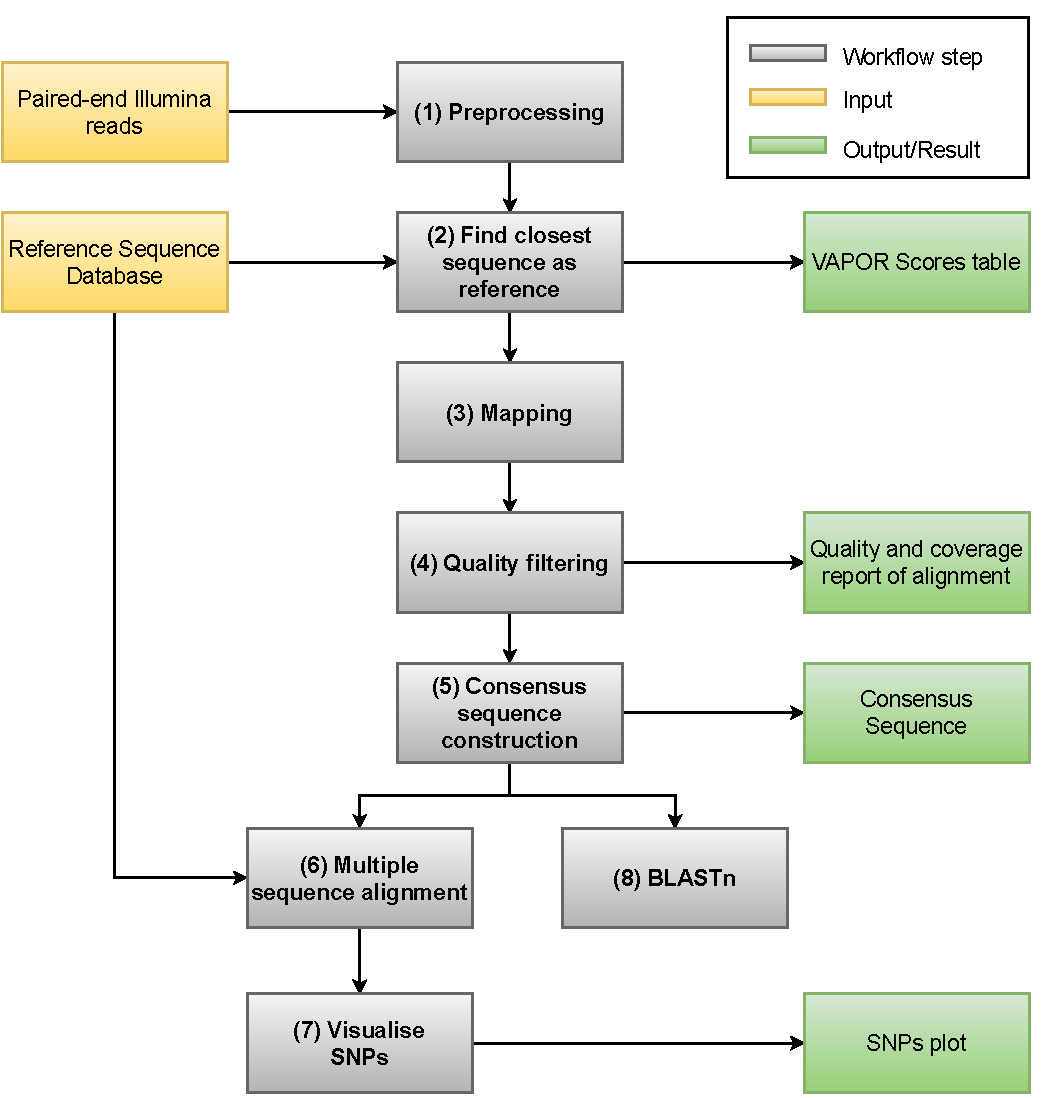
\includegraphics[width=1\textwidth]{media/3-fmdv.pdf}
	\caption{Simplified \ac{FMDV} genomic analysis workflow for Illumina-sequenced data.}
	\label{fig:3-fmdv-wf}
\end{figure}

We propose a mapping-based workflow for the analysis of data from Foot-and-mouth disease virus using Illumina sequencing technology. The workflow takes multiple samples in a collection and is integrated into the Galaxy platform. It is available with the additional material via links provided in Supplementary~\secref{sec:apx-fmdv-links}, and follows the \ac{SARS-CoV-2} workflow pattern. Its full list of steps in \ac{CWL} format can be found in Supplementary~\secref{sec:apx-fmdv-wf}. \\
The workflow starts with (1) preprocessing of the reads using \texttt{fastp}. Reads shorter than 30 base pairs are discarded, and PolyG tails of the Illumina reads are trimmed automatically. \\
The preprocessed reads are then used to find the closest possible reference sequence using \texttt{VAPOR}. As \ac{FMDV} is not a segmented virus, the reference sequence database provided for this virus consists of one FASTA file with multiple full-length sequences from different serotypes. The provided database file consists of 201 sequences, each containing the complete and N-free genome of \ac{FMDV}. The highest-scoring sequence from the \texttt{VAPOR} run is used as the reference sequence for the alignment. The highest \texttt{VAPOR} scores of each run are summarised in a table to check for the quality of the results. \\
The third step of the workflow is (3) mapping with \texttt{BWA-MEM}. Mapping of the preprocessed reads against the reference is run with default parameters of \texttt{BWA-MEM}. The resulting \ac{BAM} dataset is (4) quality filtered using \texttt{Samtools view}. Only reads with a minimum quality of 20 and those that are paired and mapped in a proper pair are kept. Alignment and quality reports including coverage statistics are generated per sample using \texttt{QualiMap BamQC}. \\
Similar to the \ac{SARS-CoV-2} workflow, (5) consensus sequence construction is run with \texttt{iVar consensus} and a minimum quality score threshold of 20, minimum frequency threshold of 0.7, minimum depth to call consensus of 10, and does not exclude regions with smaller depth than the minimum threshold. These settings accept any base as the consensus base for a genome position with a base calling quality of 20 or above. \\
After constructing the consensus sequence, (6) multiple sequence alignment of a subset of the reference sequences with the consensus sequence is performed using \texttt{MAFFT}. The size of the subset can be adapted via user input and defaults to the seven sequences with the highest \texttt{VAPOR} scoring. The \ac{MSA} is then used to visualise SNPs with \texttt{snipit}. A (7) BLASTn search is performed against a database of known FMDV serotypes to confirm the serotype of the FMDV sample and preclude contamination, co-infections or recombination. The workflow produces a summary report of the results of each step and allows the user to investigate the output of each step further for additional research. The workflow is outlined in~\ref{fig:3-fmdv-wf}.
